\documentclass[../../LearnCpp.tex]{subfiles}

\graphicspath{{\subfix{../images/}}}

\begin{document}

\asubsection{11}{Header files}

\subsubsection*{使用标准库的头文件}

\begin{figure}[bh]
   \centering
   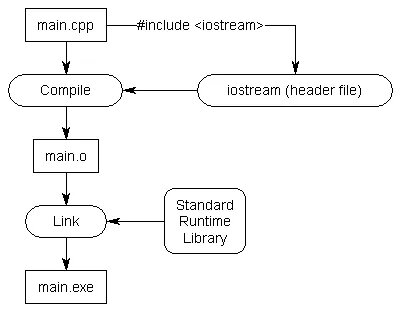
\includegraphics[width=10cm]{\subfix{../images/IncludeLibrary}}

   \label{fig:IncludeLibrary}
   \caption{IncludeLibrary}
\end{figure}

\subsubsection*{编写自定义的头文件}

add.cpp:

\begin{lstlisting}[language=C++]
int add(int x, int y)
{
   return x + y;
}
\end{lstlisting}

main.cpp:

\begin{lstlisting}[language=C++]
#include <iostream>

int add(int x, int y); // 前向声明使用函数原型

int main()
{
   std::cout << "The sum of 3 and 4 is " << add(3, 4) << '\n';
   return 0;
}
\end{lstlisting}

编写头文件非常简单,因为只包含了两部分:

\begin{enumerate}
   \item \textit{头文件保护符},下一章将会讨论。
   \item 头文件的实际内容,其应该为前置定义的标识符,使得其他文件可以看到。
\end{enumerate}

项目中添加一个头文件类似于添加一个源文件(2.8 的多文件程序将提到)。

头文件经常与代码文件配对,头文件为相关的代码文件提供前向声明。

add.h:

\begin{lstlisting}[language=C++]
// 1. 需要一个头文件保护符在这里,将在下一章讲解,这里现在暂时忽略它

// 2. 这里是 .h 文件的内容,也是声明开始的地方
int add(int x, int y); // 函数原型 add.h -- 不要忘记分号!
\end{lstlisting}

main.cpp:

\begin{lstlisting}[language=C++]
#include "add.h" // 插入 add.h 的内容到该处。注意这里使用双引号。
#include <iostream>

int main()
{
   std::cout << "The sum of 3 and 4 is " << add(3, 4) << '\n';
   return 0;
}
\end{lstlisting}

add.cpp:

\begin{lstlisting}[language=C++]
#include "add.h" // 插入 add.h 的内容到该处。注意这里使用双引号。

int add(int x, int y)
{
   return x + y;
}
\end{lstlisting}

当预处理器处理 \acode{\#include "add.h"} 行时,拷贝 add.h 的内容至当前文件的该处。
因为 \textit{add.h} 包含了函数 \textit{add} 的前向声明,前向声明将会被拷贝到 \textit{main.cpp}。
最终的结果是程序的功能与手动添加前向声明在 \textit{main.cpp} 文件顶部的效果一直。

\begin{figure}[bh]
   \centering
   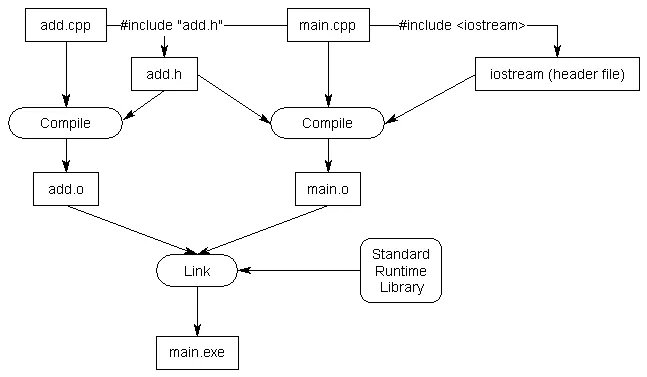
\includegraphics[width=10cm]{\subfix{../images/IncludeHeader}}

   \label{fig:IncludeHeader}
   \caption{IncludeHeader}
\end{figure}

\subsubsection*{源文件应该包含其配对的头文件}

在 C++ 中,代码文件的最佳时间是 \acode{\#include} 它们配对的头文件(如果存在的话)。上面的例子中 \acode{add.cpp} 包含了 \acode{add.h}。

\subsubsection*{尖括号 vs 双引号}

有可能会好奇为什么 \acode{iostream} 使用的是尖括号,而 \acode{add.h} 使用的是双引号。因为在不同的路径下可能存在相同名称的头文件。两种方式的使用可以帮助预处理器在何处寻找头文件。

当使用尖括号时,则是告诉预处理器该头文件不是由用户编写的。预处理器将会寻找只指定于 \acode{include directories} 路径下的头文件。\acode{include directories} 由用户的项目/IDE 设置/编译器设置配置,通常默认路径中的头文件由用户编译器和/或操作系统所包含。预处理器不会在项目的源代码路径中寻找。

当使用双引号时,则是告诉预处理器头文件是由用户编写的。预处理器将会首先寻找当前路径。如果不能找到匹配的头文件,则会再从 \acode{include directories} 中寻找。

\subsubsection*{头文件可能包含其他的头文件}

最佳实践:

每个文件应该显式的 \acode{\#include} 所有其需要编译的头文件。不要依赖包含了其他头文件的头文件。

\subsubsection*{头文件的 \#include 顺序}

最佳实践:

为了最大化编译器发现缺失的 includes,请按照以下顺序进行 \#includes:

\begin{enumerate}
   \item 匹配的头文件
   \item 本项目中其他的头文件
   \item 第三方库的头文件
   \item 标准库的头文件
\end{enumerate}

其中每个组的头文件根据字母顺序进行排序。

这样的话,如果用户自定义的头文件缺失了三方库或者标准库的 \#include,则很可能会产生编译错误,因此可以进行修复。

其他的最佳实践:

\begin{itemize}
   \item 总是包含头文件保护符(详见下一章节)
   \item 不要在头文件中定义变量以及函数(全局变量除外 -- 之后的章节将会覆盖)
   \item 头文件和与之关联的源文件拥有一样的名字(例如 grades.h 用于匹配 grades.cpp)
   \item 每个头文件需要有特定的任务,并且越独立越好。
         例如用户讲所有关联 A 功能的声明放入 A.h 中,所有关联 B 功能的声明放入 B.h 中。
         这样用户只需要关心 A 时 include A.h,而不会获得任何关联 B 的事务
   \item 注意头文件需要显式的在代码文件中 include 所需要的功能
   \item 所有用户编写的头文件应该可以自身被编译(应该 \#include 所有其所需的依赖)
   \item 仅 \#include 所需要的
   \item 不要 \#include .cpp 文件
\end{itemize}

\end{document}
